\section{Introduction}

Nowadays, the number of open datasets from different organizations ($e.g.,$ governments and companies) keeps growing, providing immense opportunities for intelligent data analysis. However, these datasets are usually stored in a data lake which is not as well-organized as a relational database with well-defined schemes and indexes. Hence, it is challenging to efficiently and effectively find the data required by users, given the scale of data lake and the semantics of user requirements. \lei{What does the semantics of user requirement mean?} 
To exploit the enormous value in the data lake, researchers from both academia and industry and have developed a number of data discovery engines~\cite{} that retrieve relevant tables based on users' need. 

\begin{figure*}[h]
	\centering
	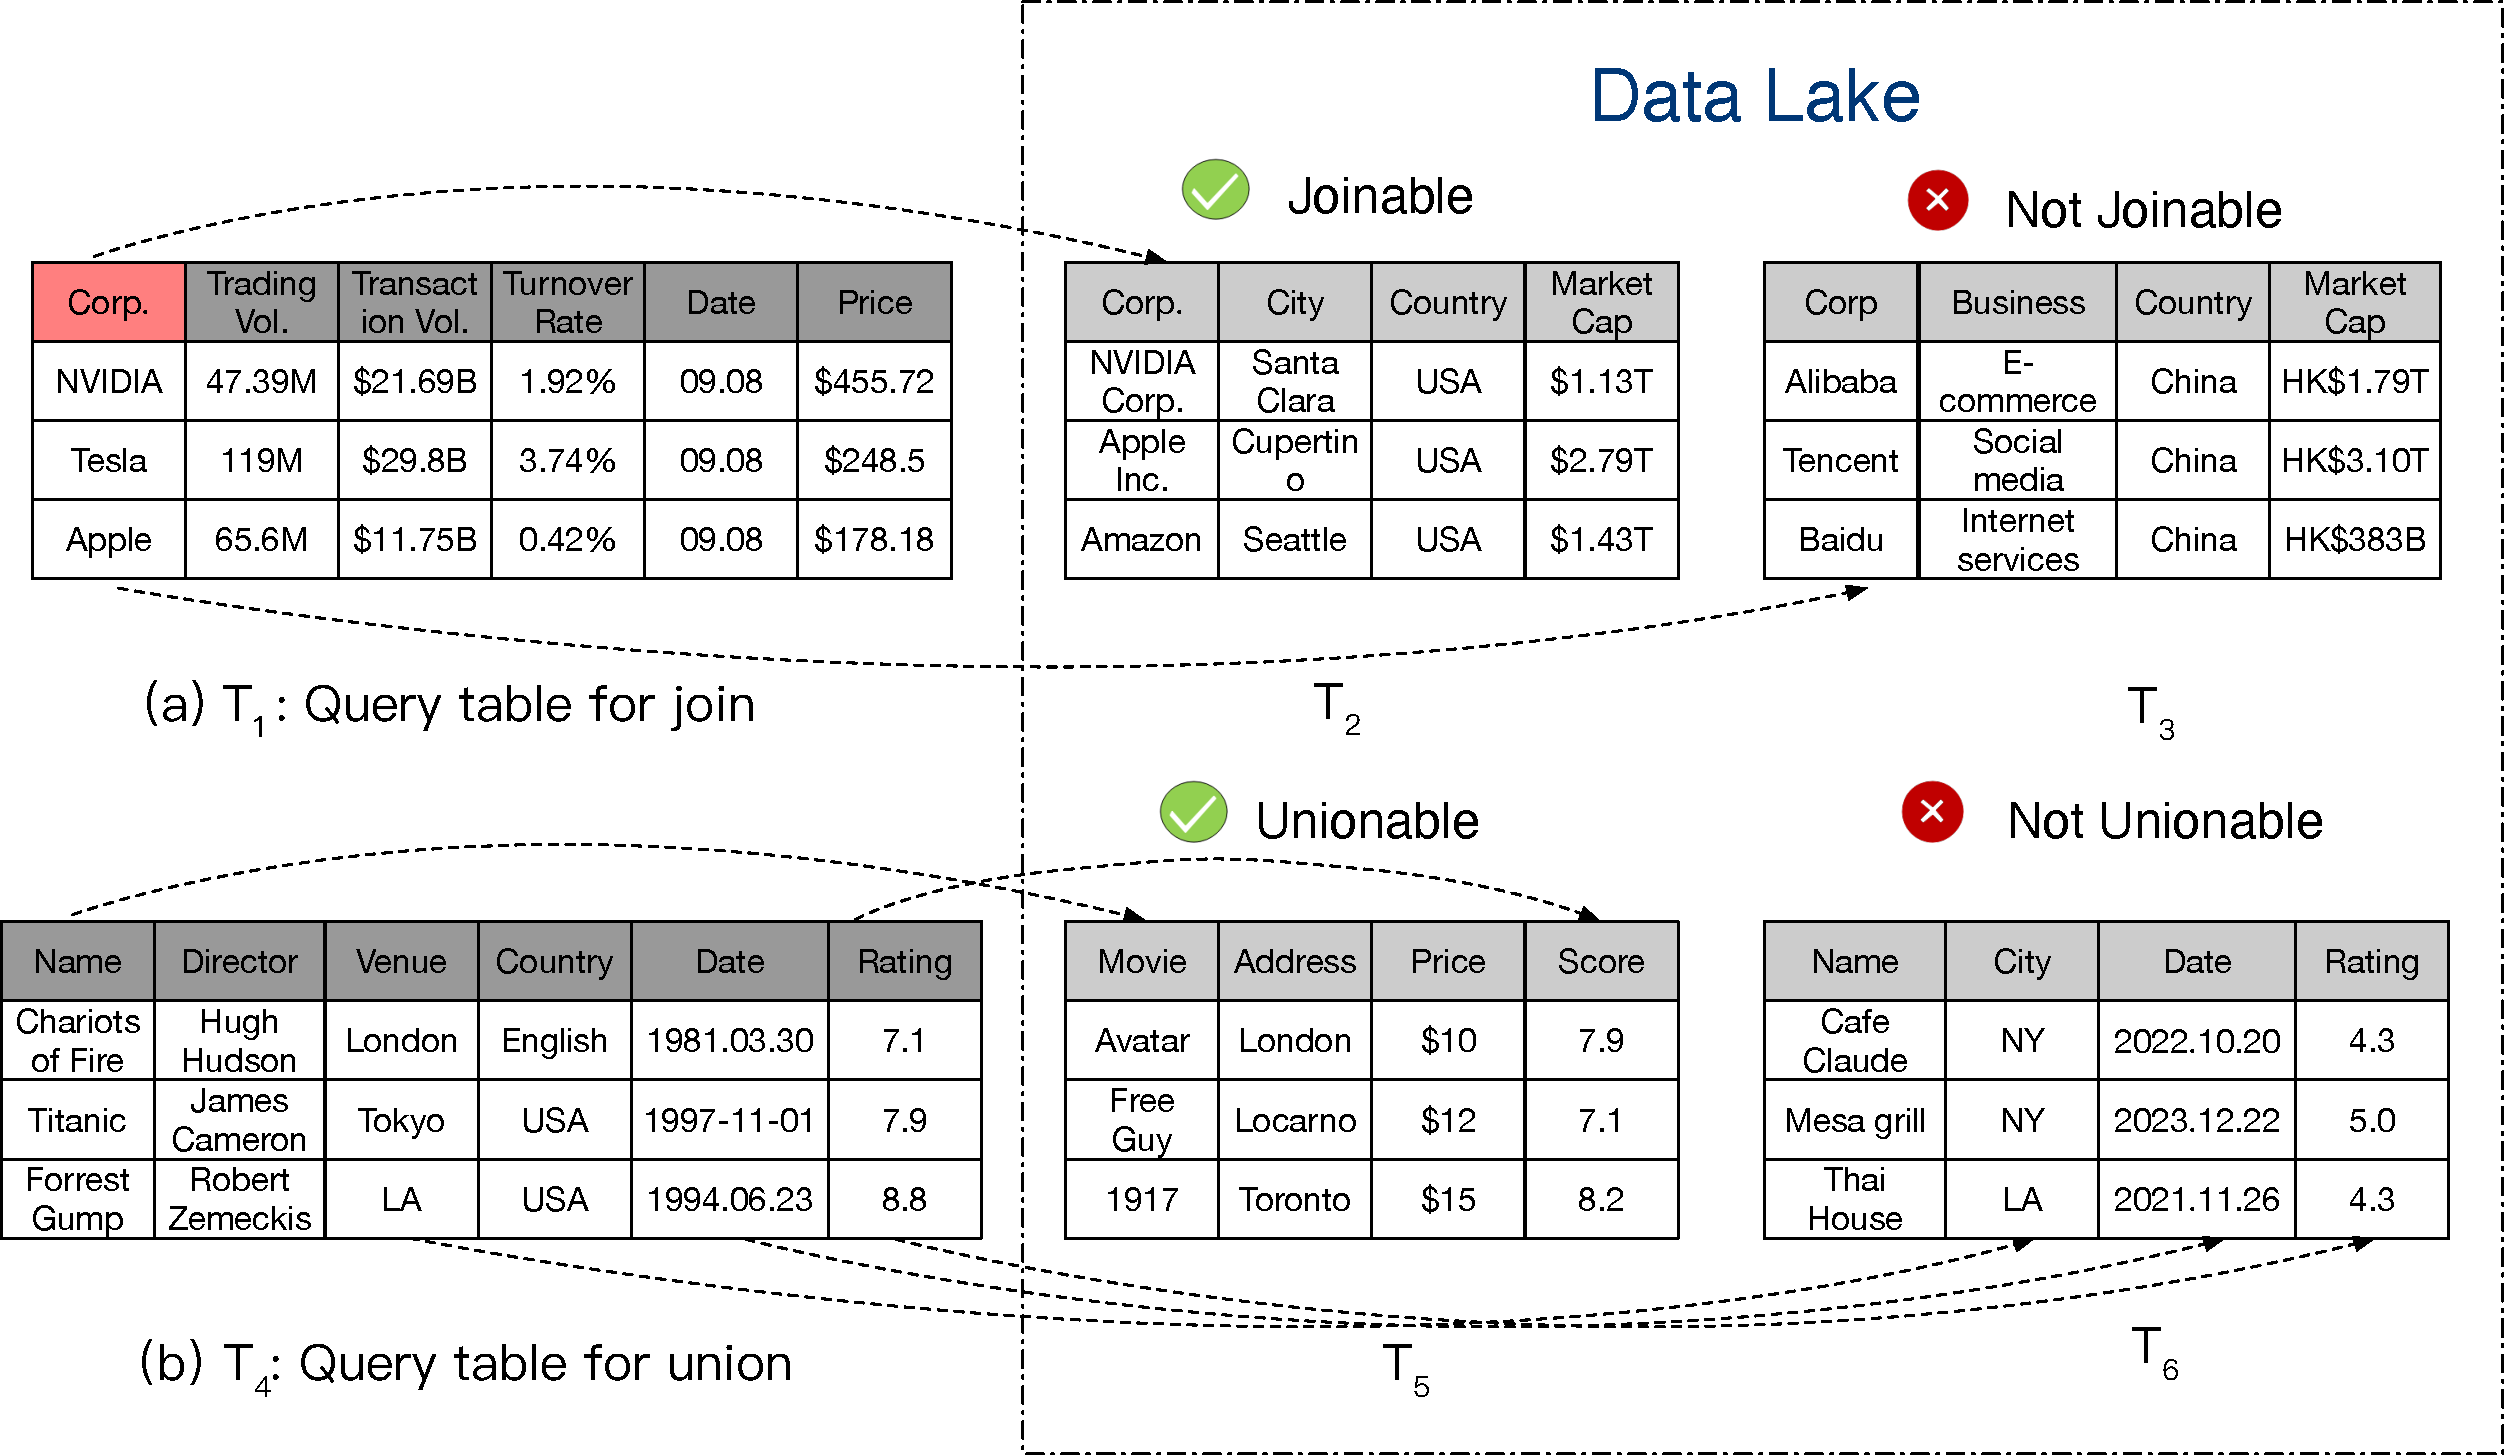
\includegraphics[width=0.8\linewidth]{fig/example.pdf}
	\caption{Table Discovery in Data Lake.}
	\label{fig:example}
\end{figure*}


%given a query table, they search relevant tables from the data lake, so as to benefit the downstream applications, such as augmenting more data instances~\cite{} or  improving the machine learning model performance~\cite{}. 

The general task of discovering tables from data lakes can be classified into several categories, \eg keyword-based search, joinable table search and unionable table search. Among these categories, keyword-based search~\cite{} issues {\it a set of keywords} as queries to retrieve relevant tables, while joinable and unionable table searches issue a {\it table} as the query.
In this work, we focus on the latter two categories, because recently they have attracted much attention in data management field to augment data instances~\cite{} or tuples~\cite{}, so as to  benefit the downstream applications like machine learning based data analysis. 
%

More specifically, given a query table with a user-specified column, joinable table search finds the target tables that can be joined with the column.

\begin{example}
	As shown in Figure~\ref{fig:example}(a), given the query table ($T_1$) and a specified column \texttt{Corporation}, Table $T_2$ in the data lake is joinable with $T_1$, \ie the first attribute of $T_2$ can be joined with the specified column because i). the column names match and ii). a number of cell values semantically overlap (\eg Apple and Apple Inc.). 
	%
	The joined table improves model performance when the \texttt{Price} is treated as the predicted column because of the augmented features.
	%
	On the other hand, although in $T_3$, the column name and the contents of its first attribute are semantically similar with the specified column, it is not joinable because there is no overlapping value.
\end{example}

For unionable table search, given a query table, it aims to find target tables that are unionable with the query.                  

\begin{example}
	As shown in Figure~\ref{fig:example}(b), given a query table ($T_4$), $T_5$ can be unioned with $T_4$ because they are all about the information of movies and two pairs of attributes are highly correlated ($T_4$.\texttt{Name} $v.s.$ $T_5$.\texttt{Movie} and $T_4$.\texttt{Rating} $v.s.$ $T_5$.\texttt{Score}). 
	However, when it comes to $T_6$ which has three attributes ($T_6$.\texttt{City}, $T_6$.\texttt{Date} and $T_6$.\texttt{Rating}) and are aligned respectively with attributes ($T_4$.\texttt{Venue}, $T_4$.\texttt{Date} and $T_4$.\texttt{Rating}) of $T_4$,  $T_6$ is not unionable with the query $T_4$. This is because the two tables are not semantically relevant ($T_4$ is about movies, while $T_6$ is about restaurants).
\end{example}

Based on the above examples, clearly table discovery is a challenging task because we have to take multiple key factors into consideration, including: (1) the (semantic) schema similarity of columns, (2) the (semantic) overlap between columns, and (3) the contextual information of all columns in a table. \lei{We don't mention contextual information before.}
What's more, as a data lake is typically large-scale, designing efficient and scalable discovery algorithms is critical yet challenging \lei{due to the high complexity of this problem}.

Due to the importance of table discovery, a range of approaches have been proposed to address the above problems from different perspectives. However, these approaches are yet to be thoroughly evaluated due to the lack of a comprehensive benchmark. 
In retrospect, benchmarks have played a significant role in spawning the boom in different research communities, such as
TPC benchmarks~\cite{} for the database community, ImageNet~\cite{} for computer vision tasks, and GLUE~\cite{} for natural language processing tasks. \lei{Not sure if we need the last sentence.}


\nan{
	\bi
	\item Intro
	\be
	\item Sec~1 Add a table or several tables to compare the number of tables/queries supported by your benchmark and others'. 
	\item Easy-to-use APIs: maybe you can give examples for designed unified APIs, saying learned from Hugging Face. They can easily compare different methods. 
	\item Leaderboard.
	\ee
	\item Sec~3 Benchmark design: align with the revised intro
	\item Sec~4 Statistics of datasets, Sec~5 Statistics of queries -- they can be merged if each section is short
	\item Annotation process
	\item API design can be pushed before ``Analyzing benchmark results''
	\ei
}

%builds a benchmark for table union search, which contains around 5,000 tables (from OpenData), among which 1,000 queries are selected as query tables with ground truth.
%that uses two data lakes. One is the same with TUS, and the other is sampled from the Web Table, with 1,000 query columns respectively, 

Santos~\cite{Santos} improves the TUS benchmark by additionally labeling column-to-column relations to consider more semantics, but it only targets table union search with around 10,100 data lake tables and 80 query tables.

\noindent \textbf{Existing Benchmarks.} All existing benchmarks have big limitations. 
TUS~\cite{TUS} and Santos only target table union search. \lei{Moreover, their data lakes are not large enough. With at most 10,100 tables and xx G data, it is not sufficient to evaluate the efficiency and scalability of the discovery algorithms.}
\lei{On the other hand, Josie~\cite{Josie} is a join search benchmark. However, it only targets evaluating the efficiency of the exact join-based search algorithms, while the effectiveness is overlooked.} 
%Valentine~\cite{valentine} evaluates multiple schema matching techniques to solve table discovery tasks, using several hundreds of tables to match pairs of tables. A recent Arxiv work~\cite{arxiv} focuses on evaluating table pretraining methods for table discovery tasks, with the goal of improve downstream machine learning tasks. 


\noindent \textbf{Challenges.} Comprehensively benchmarking table discovery faces several major challenges.

\cc{\noindent (1) [\textit{Data/Query Coverage}] The effectiveness and efficiency of table discovery largely rely on the characteristics of datasets, like the data lake scale, average column/instance number per table etc. Also, different query  characteristics also lead to different performance, such as query column/table size,  query column type,  result size etc. }

\noindent (2) [\textit{Ground Truth Labeling}] 
Most existing benchmarks have limited number of queries,  mainly because it is rather expensive to label the ground truth (tables  that can join/union with query in data lake) for each query table. Hence, it is non-trivial to create sufficient queries with ground truth to evaluate different table search approaches.

\noindent (3) [\textit{Solution Coverage}] 
Recently, several unionable/joinable table search methods have been proposed, but there lacks of a thorough comparison over these methods.

\noindent (4) [\textit{User-friendly Interface for Benchmark Usage}] Existing benchmarks just provide datasets, queries and ground truth, which is not very user-friendly if a user wants to
run different algorithms over these benchmarks.

In this paper, we propose to create a benchmark \sys that addresses all above challenges.

First, we collect 1 TB tables from two sources, namely OpenData~\cite{} and  WebTable~\cite{}, on which we evaluate different table union/join search approaches. The two sources have diverse characteristics. WebTable has a large number of tables (XXX) but each table is small. In contrast, openData consists of large tables (at least XXX) but has fewer tables than WebTable. 

\lei{How many tables and queries do we have? I agree with Boss Tang that a table with these numbers will be very helpful.}
Second, we create sufficient number of diverse queries using two approaches. In the first approach we split big tables in data lake into small ones and put these small tables into the data lake, which are joinable or unionable. Naturally, we automatically get the ground truth when these small tables serve as queries. 
Moreover, we directly use real tables from the data lake as queries. This indicates that we have to spend much efforts on labeling their ground truth.
To improve the labeling accuracy and minimize human efforts, we implement a labeling platform and design a candidate generation strategy to improve the recall \lei{What does improving recall mean here?}.   

%Third, we evaluate various approaches~\cc{\cite{}}, including techniques like schema matching, local sensitive hash,  pre-trained language models etc. for joinable/unionable table search on our benchmark datasets, so as to provide meaningful insights for scalability and accuracy of different approaches on different datasets.

\lei{It is not super clear to me what key information we want to convey here. So I re-wrote it.}
\lei{Third, we implement many key techniques such as schema matching, local sensitive hash,  pre-trained language models etc., which are the building blocks of various table discovery approaches, making sure that we are able to evaluate the scalability and accuracy of various joinable/unionable table search approaches on different datasets.}


Fourth, we implement an easy-to-use API which enables a user to conveniently issue join/union table queries and contrast the results of multiple state-of-the-art discovery approaches, through a few lines of python code. Figure~\ref{fig:api} shows the example.

Table~\ref{Table:benchmarks} compares \sys against existing benchmarks. Out of OpenData~\cite{} and  WebTable~\cite{}, we build 4 data lakes (corresponding to the gray rows), over which  both join and union search are performed. \sys is a more comprehensive benchmark because of the much larger number of queries with various characteristics and much larger data lake size. Therefore, both the effectiveness and efficiency of different table discovery algorithms are thoroughly evaluated. 

\begin{figure}[h]
	\centering
	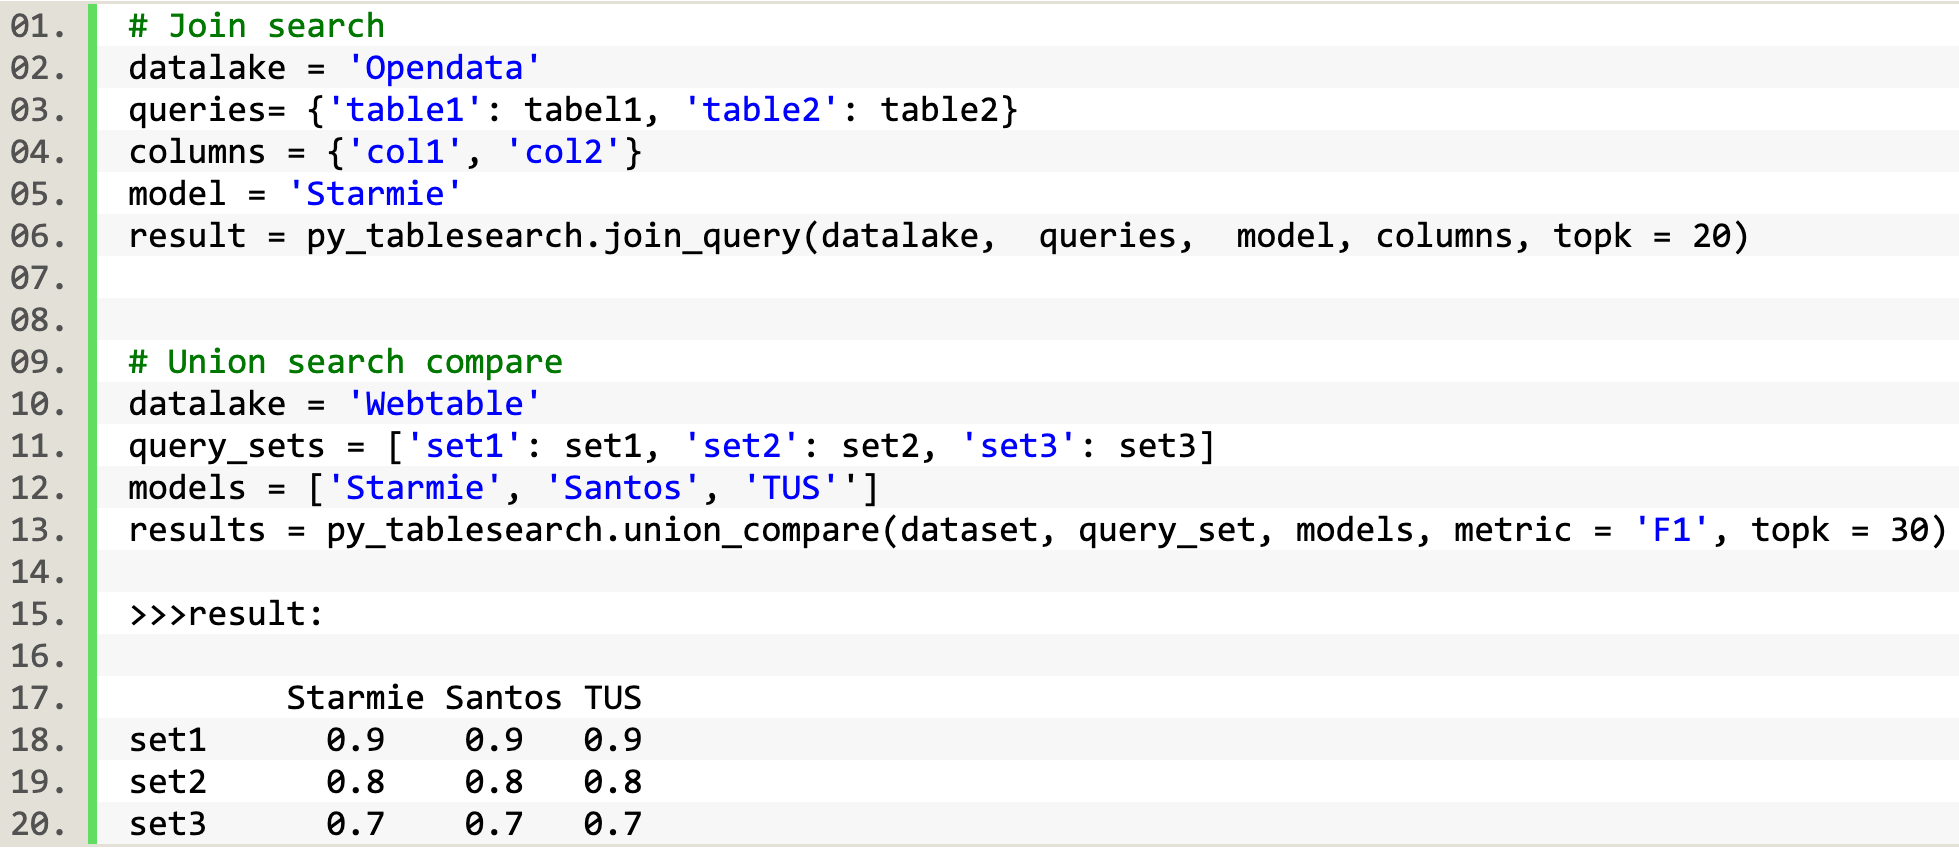
\includegraphics[width=\linewidth]{fig/api}
	\caption{API Example.}
	\label{fig:api}
\end{figure}

To summarize, we make the following contributions.

\noindent (1) We build a comprehensive benchmark, \sys, for table discovery in data lake, including large-scale datasets, sufficient and various queries, as well as thorough evaluation.  

\noindent (2) We collect more than 1 TB real tables from multiple sources, indexing them with different strategies for table search with different approaches.  

\noindent (3) We create various query tables covering different characteristics, and accurately label ground truth for them.

\noindent (4) We evaluate and analyze multiple state-of-the-art joinable/unionable table search approaches using these created queries on the benchmark datasets.

\noindent (5) We build a use-friendly API to well support table search in data lakes. 


\begin{table*}[t]
	\centering
	\caption{Benchmark Comparison.}
	\setlength{\arrayrulewidth}{0.5pt} % 增加线宽
	\begin{tabular}{|c|c|c|c|c|c|c|}
		\hline
		\centering
		Benchmarks & Type & $\#$-Query tables & $\#$-Lake tables & $\#$-Total columns & Size (GB) &  API \\
		\hline  
		TUS Small~\cite{TUS}& Union  & 200 & 1,530 & 14,810 & 1 & \XSolidBrush \\
		\hline
		TUS Large~\cite{TUS}& Union  & 1,000 & 5,043 & 54,923 & 1.5 & \XSolidBrush \\
		\hline
		Santos Small~\cite{Santos}& Union  & 50 & 550 & 6,322 & 0.45 & \XSolidBrush \\
		\hline
		Santos Large~\cite{Santos}& Union  & 80 & 11,090 & 123,477 & 11 & \XSolidBrush  \\
		\hline
		Josie~\cite{Josie}& Join  & XX & XX  & XX  & XX &  \XSolidBrush \\
		\hline
		%Valentine~\cite{valentine}& XX  & XX & XX  & XX  & XX &  \XSolidBrush \\
		%\hline
		%LakeBench~\cite{arxiv}& Union & XX & XX  & XX  & XX &  \XSolidBrush \\
		%\hline
		\rowcolor{gray!40} 
		OpenData Small & Join \& Union  & 3,173 & 10,374  & 166,770  & 100.03 & \Checkmark  \\
		\hline
		\rowcolor{gray!40}
		OpenData Large & Join \& Union  & XX & 64,698  & 1,357,758  & 1111.40 & \Checkmark  \\
		\hline
		\rowcolor{gray!40}
		WebTable Small & Join \& Union  & 5,826 & 2,772,825  & 17,929,497  & 13.01 & \Checkmark\\
		\hline
		\rowcolor{gray!40}
		WebTable Large & Join \& Union  & XX & 16,684,293  & 107,891,225  & 77.05 &\Checkmark \\
		\hline
	\end{tabular}
	\label{Table:benchmarks}
	
\end{table*}
